\section{Auswertung}
\label{sec:Auswertung}


\subsection{Blockschaltbild}
\subsection{Grafische Darstellung der Stackspannung, der
Stackleistung, der Verbraucherleistung und des Wasserstoffverbrauchs}
\begin{figure}[H]
    \centering
    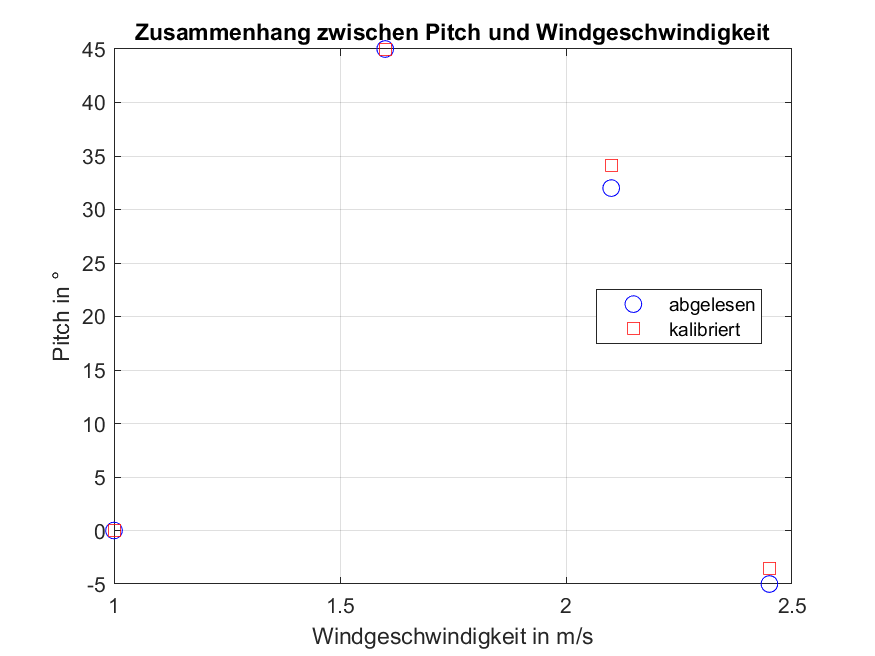
\includegraphics[width=0.8\textwidth]{plot1}
    \caption{Grafische Darstellung der Stackspannung, der
    Stackleistung, der Verbraucherleistung und des Wasserstoffverbrauchs.}
    \label{fig:plot1_26062023}
  \end{figure}
\subsection{Grafische Darstellung einiger Messgrößen im Bezug zum Verbracuherstrom}
\begin{figure}[H]
    \centering
    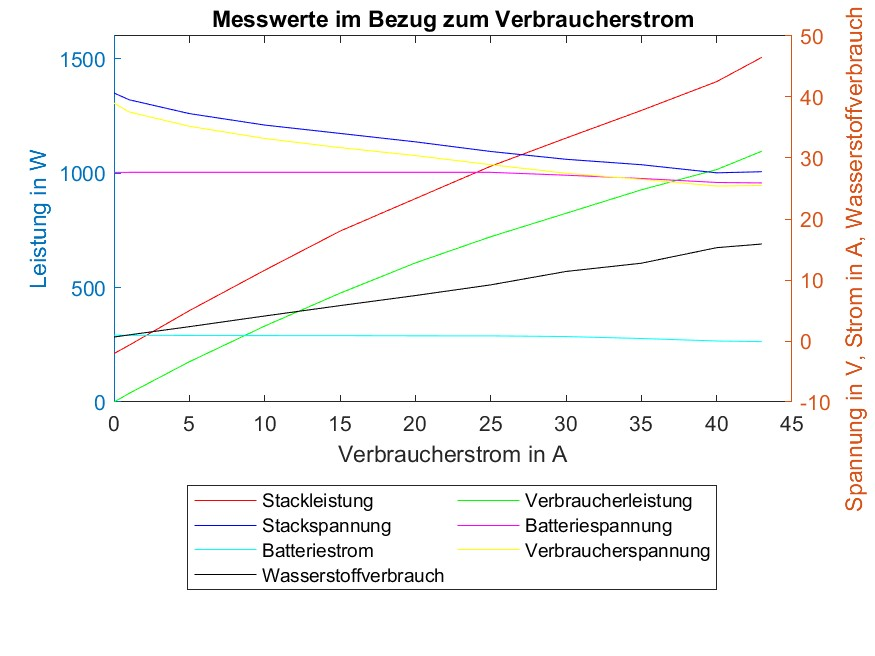
\includegraphics[width=0.8\textwidth]{grafik2}
    \caption{Grafische Darstellung der Stackspannung, der
    Stackleistung, der Verbraucherleistung und des Wasserstoffverbrauchs.}
    \label{fig:plot2_26062023}
  \end{figure}
  \begin{figure}[H]
    \centering
    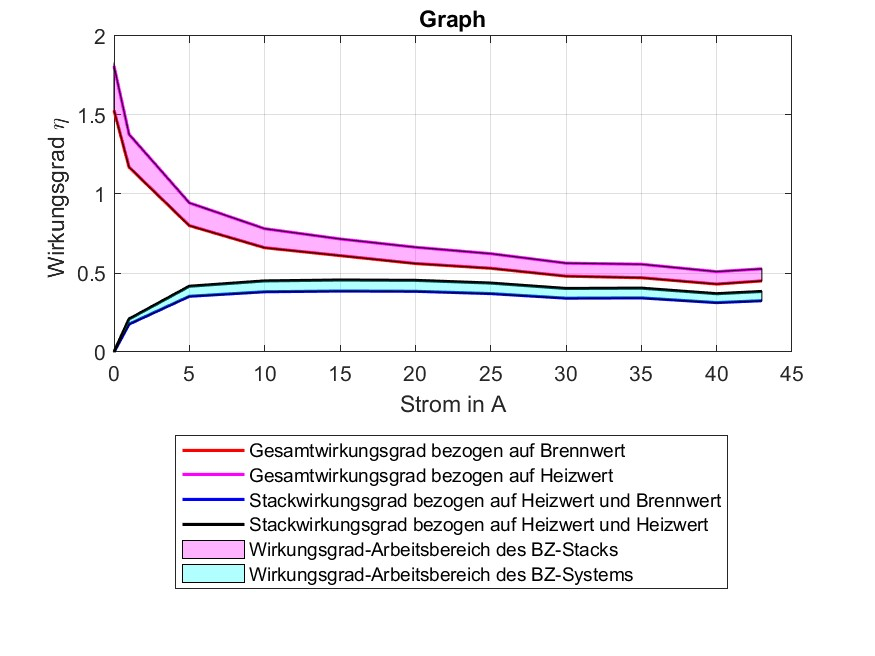
\includegraphics[width=0.8\textwidth]{plot3}
    \caption{Grafische Darstellung der Stackspannung, der
    Stackleistung, der Verbraucherleistung und des Wasserstoffverbrauchs.}
    \label{fig:plot3_26062023}
  \end{figure}
\subsection{Diskussion der Kurven}
\subsection{}
\subsection{Teillastverhalten}

Leistung prinzipiell mit höherer Temperatur größer, außerdem Batteriestrom höher? 
Steigt der Teillastwirkungsgrad mit steigender Temperatur (nicht über betriebstemperatur) oder ist das unsinnig?
Warum ist der Batteriestrom auf einmal so hoch? Puffert die Batterie die Leistung aus die nicht mehr von der BZ bereitgestellt werden kann durch die höhere temperatur?



\subsection{Energiebilanz für den Teillastfall}